% ===================== PACKAGES =====================
\usepackage[british]{babel}
\usepackage[tmargin=1in, bmargin=1in, lmargin=0.75in, rmargin=0.75in]{geometry}
\usepackage[dvipsnames,table]{xcolor}  % prima di tikz, listings, ecc.

\usepackage{tikz}
\usepackage{graphicx}
\usepackage{pgfplots}
\pgfplotsset{width=12cm, compat=1.9}
\usepackage{setspace}
\usepackage{chemmacros}
\usepackage{chemfig}
\usepackage{esint}
\usepackage{tabularray}
\usepackage{makeidx}
\usepackage{epstopdf}
\usepackage{amssymb}
\usepackage{mathrsfs}
\usepackage{bm}
\usepackage{amsmath}
\usepackage{enumitem}
\usepackage[english]{varioref}
\usepackage{lipsum}
\usepackage{fancyhdr}
\usepackage{float}
\usepackage{empheq}
\usepackage[framemethod=tikz]{mdframed}
\numberwithin{equation}{section}
\usepackage{eso-pic}
\usepackage{calc}
\usepackage{nccmath}
\usepackage{caption}
\usepackage{subcaption}
\usepackage{gensymb}
\usepackage{amsfonts, amsthm, epsfig, epstopdf, titling, url, array}
\usepackage{tabularx}
\usepackage{makecell}
\usepackage{booktabs}
\usepackage{array}
\usepackage{siunitx}
\sisetup{input-digits=0123456789\pi}
\usepackage[symbol]{footmisc}
\usepackage{multicol}
\usepackage{boondox-cal}
\usepackage{blindtext}
\usepackage{changepage}
\usepackage{nomencl}
\usepackage{hyperref}
\usepackage{xurl}
\usepackage{ragged2e}
\usepackage[version=4]{mhchem}  % ← conflitto di opzioni
\usepackage{longtable}
\usepackage{chemformula}

% ===================== SI UNITS =====================
\DeclareSIUnit\atm{atm}
\DeclareSIUnit{\var}{var}
\DeclareSIUnit{\pu}{p.u.}


% ===================== MATH OPERATORS =====================
\DeclareMathOperator{\rank}{rank}
\DeclareMathOperator{\atantwo}{atan2}
\DeclareMathOperator{\spn}{span}

% ===================== COMMANDS =====================
\newcommand{\abs}[1]{\left|#1\right|}
\newcommand{\sign}{\text{sign}}
\newcommand{\centered}[1]{\begin{tabular}{@{}l@{}} #1 \end{tabular}}

% ===================== COLORS =====================
\definecolor{mycolor1}{rgb}{0.97, 0.97, 0.97}
\definecolor{mycolor2}{rgb}{0.97, 0.97, 0.97}
\definecolor{tableShade}{gray}{0.9}

% ===================== THEOREM ENVIRONMENTS =====================
\theoremstyle{it}
\newtheorem{defn}{Definition}[section]
\newtheorem{assumption}{Assumption}[section]
\newtheorem{thm}{Theorem}[section]
\newtheorem{lemma}{Lemma}[section]
\newtheorem{corollary}{Corollary}[section]
\theoremstyle{definition}
\newtheorem{example}{Example}[section]

% ===================== CUSTOM ENVIRONMENTS =====================
\newenvironment{myitemize_1}{
	\begin{itemize}[topsep=0pt]
		\setlength{\topsep}{2pt}
		\setlength{\itemsep}{2pt}
		\setlength{\parskip}{2pt}
		\setlength{\parsep}{2pt}
	}{\end{itemize}}

\newmdenv[
innerlinewidth=0.5pt,
roundcorner=4pt,
backgroundcolor=mycolor2,
linecolor=mycolor1,
innerleftmargin=6pt,
innerrightmargin=6pt,
innertopmargin=6pt,
innerbottommargin=6pt
]{mybox}

% ===================== TABLE COLUMN TYPES =====================
\newcolumntype{Y}{>{\hsize=2\hsize}X}
\newcolumntype{Z}{>{\centering\arraybackslash\hsize=0.857\hsize}X}

% ===================== SECTION DEPTH =====================
\setcounter{secnumdepth}{3}
\setcounter{tocdepth}{3}

% ===================== PAGE STYLE =====================
\setlength{\headheight}{20pt}
\setlength{\headsep}{20pt}

\pagestyle{fancy}
\fancypagestyle{firstpage}{\rhead{}}
\fancyhead[L]{\slshape\nouppercase{\leftmark}}
\chead{}
\rhead{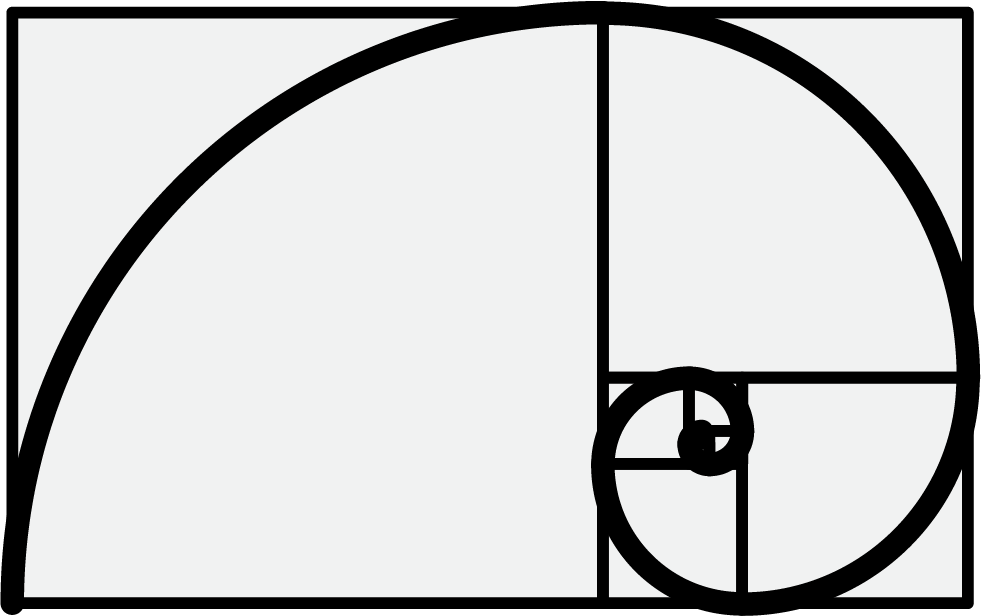
\includegraphics[height=0.75cm]{../AAA_template_latex_settings/pwr-control_logo_doc.png}}
\lfoot{\href{http://www.pwr-control.com}{pwr-control.com}}
\cfoot{-\ \thepage\ -}
\rfoot{\textit{}}
\renewcommand{\headrulewidth}{0.4pt}
\renewcommand{\footrulewidth}{0.4pt}


\geometry{
	a4paper,
	top    = 2.5cm,
	bottom = 3.0cm,
	left   = 2.5cm,
	right  = 2.5cm
}

\hypersetup{
	colorlinks = true,
	urlcolor   = blue,
	linkcolor  = black,
	citecolor  = black
}

\pagenumbering{gobble}